\chapter{Introduction}
\label{chap:intro}
\chaptermark{Optional running chapter heading}

In a classical uniform multicore\footnote{We do not distinguish terms ``multiprocessor" and ``multicore"} scheduling, an operating system scheduler allocates available uniform cores to dynamically arriving programs~\cite{Anderson2006}. Once the number of pending programs exceeds the number of cores, a scheduler prioritizes programs by either static priorities set by a system designer, or specific dynamically computed priorities. Schedulers objectives are the minimization of the average programs execution time, latency, migrations and preemptions number, and other. We emphasize that the problem of an optimal multicore scheduling is shown to be $\mathsf{NP}$-hard, and thus the heuristic approaches are typically used to find a suboptimal solution.

\section{Heterogeneous scheduling}
Even further, unlike the classical homogeneous case, heterogeneous scheduling is significantly complicated by the presence of multiple types of processing units for a computing heterogeneous hardware platform~\cite{Radulescu2000}. Some of these heterogeneous units are slow but energy efficient, while others are fast but too energy consuming (see Fig.~\ref{fig:heteroExampleOverview}). A well-known example of a heterogeneous platform is ARM big.LITTLE architecture~\cite{Padoin2015}, conceptually depicted in Fig.~\ref{fig:bigLITTLEArchitecture}. It consists of:
%
\begin{itemize}
\item a cluster of fast (``big") but energy-hungry cores;
\item a cluster of slow (``LITTLE") but energy-efficient  cores;
\item GPU and
\item NPU devices.
\end{itemize}
%
Observe the performance comparison of ``big" (Cortex-A15) and ``LITTLE" (Cortex-A7) cores in Fig.~\ref{fig:CortexA15A7Comparison}. There is an intersecting performance range for these core types, where the use of ``LITTLE" cores leads to much lower energy consumption than the use of ``big" cores.
An appropriate allocation of these processing units depends on programs activity. For example, read of 32 bytes from an 8KB SRAM consumes 125 times less energy than from a DRAM~\cite{Hennessy2017}.
%, while the SRAM read uses 50 times as much as a 32-bits integer addition. 
Considering a memory-intensive program, processing units optimized for memory access, for example, by providing larger caches, significantly reduce energy consumption at little performance degradation. Thus, a heterogeneous scheduler not only aims at optimizing time-related aspects, but also the overall energy consumption. This problem of an optimized heterogeneous scheduling is especially relevant for systems with autonomous power supplies. We elaborate on heterogeneous hardware in Section~\ref{sec:heterogeneousCase}.

\begin{figure}
\centering
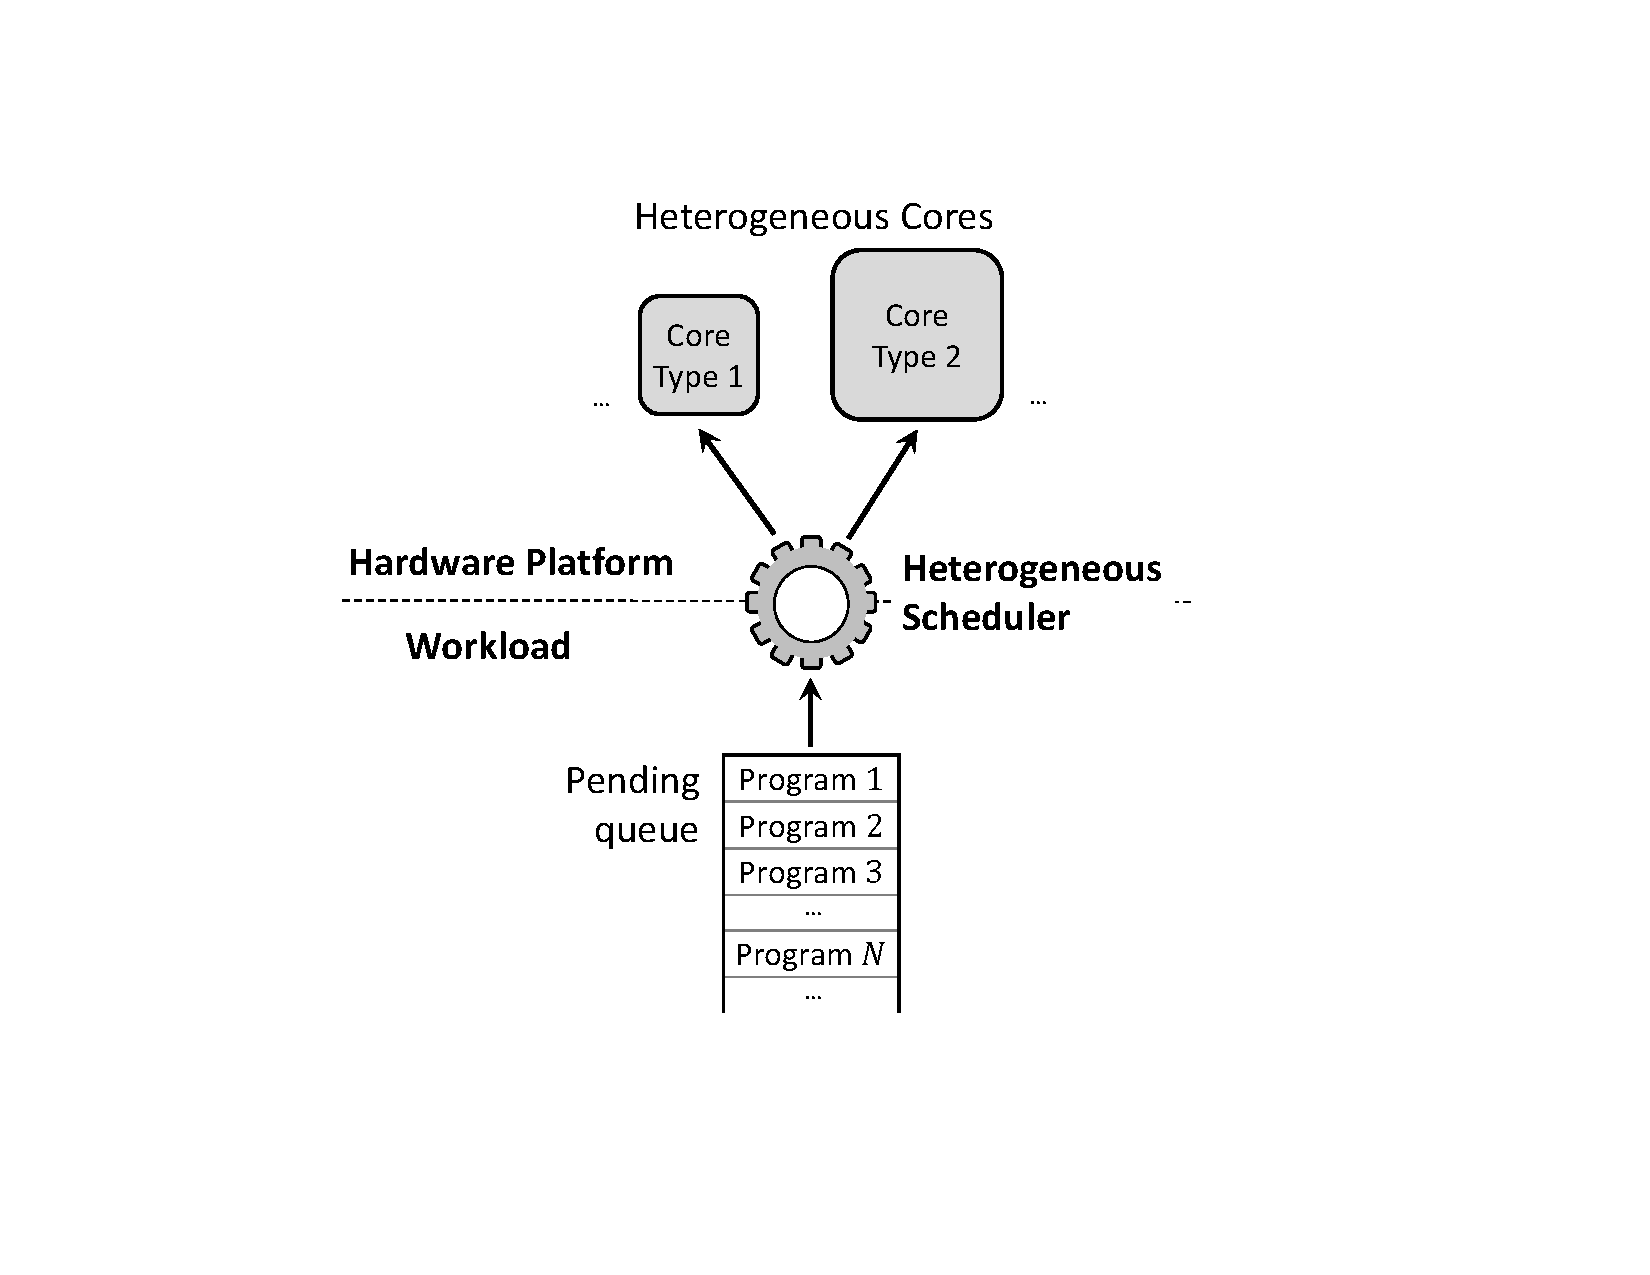
\includegraphics[width=0.5\columnwidth]{figs/heteroExampleOverview.pdf}
\caption{Heterogeneous scheduling: key components}
\label{fig:heteroExampleOverview}
\end{figure}

\section{Toy schedule example} 

Let us next provide a toy example of scheduling three programs over a heterogeneous hardware platform with one ``slow" and one ``fast" core. We assume that programs are composed of individual logically separated code blocks\footnote{The notion of a block is not yet defined and to be elaborated later. So far, we assume that program blocks execute sequentially.} with their execution requirements listed in Table~\ref{tab:demandExample}. In Fig.~\ref{fig:s1} and~\ref{fig:s2} we depict cores load and programs execution for two possible schedules S1 and S2, assuming programs arrive asynchronously at times 0, 1, and 3 respectively. For example, in S1 the ``slow'' Core 1 is allocated to the Programs 1 and 3, while in S2 this core solely executes all blocks of Program 2.

\begin{table}
\centering
\captionsetup{justification=centering}
\caption{Programs execution requirements per their block}
\label{tab:demandExample}
\begin{tabular}{|c|c|c|c|c|c|}
\hline
\multicolumn{2}{|c|}{\multirow{2}{*}[-1ex]{\makecell{Programs \\ Blocks}}} & \multicolumn{2}{c|}{Execution time, sec} & \multicolumn{2}{c|}{Energy use, Joules} \\[2pt] \cline{3-6}
\multicolumn{2}{|c|}{} & \makecell{Core 1 \\ (slow)} & \makecell{Core 2 \\ (fast)} & Core 1 & Core 2 \\ \hline
\multirow{2}{*}{P1} & B1 & 4 & 3 & 8 & 9 \\[2pt] %\cline{2-6}
 & B2 & 5 & 3 & 3 & 4 \\[2pt] \hline
\multirow{3}{*}{P2} & B1 & 5 & 4 & 6 & 10 \\[2pt] %\cline{2-6}
 & B2 & 3 & 2 & 3 & 7 \\[2pt] %\cline{2-6}
 & B3 & 3 & 2 & 3 & 6 \\[2pt] \hline
P3 & B1 & 3 & 2 & 6 & 7 \\[2pt] %\hline
 \hline
\end{tabular}
\end{table}

\begin{figure*}
\begin{subfigure}{.85\columnwidth}
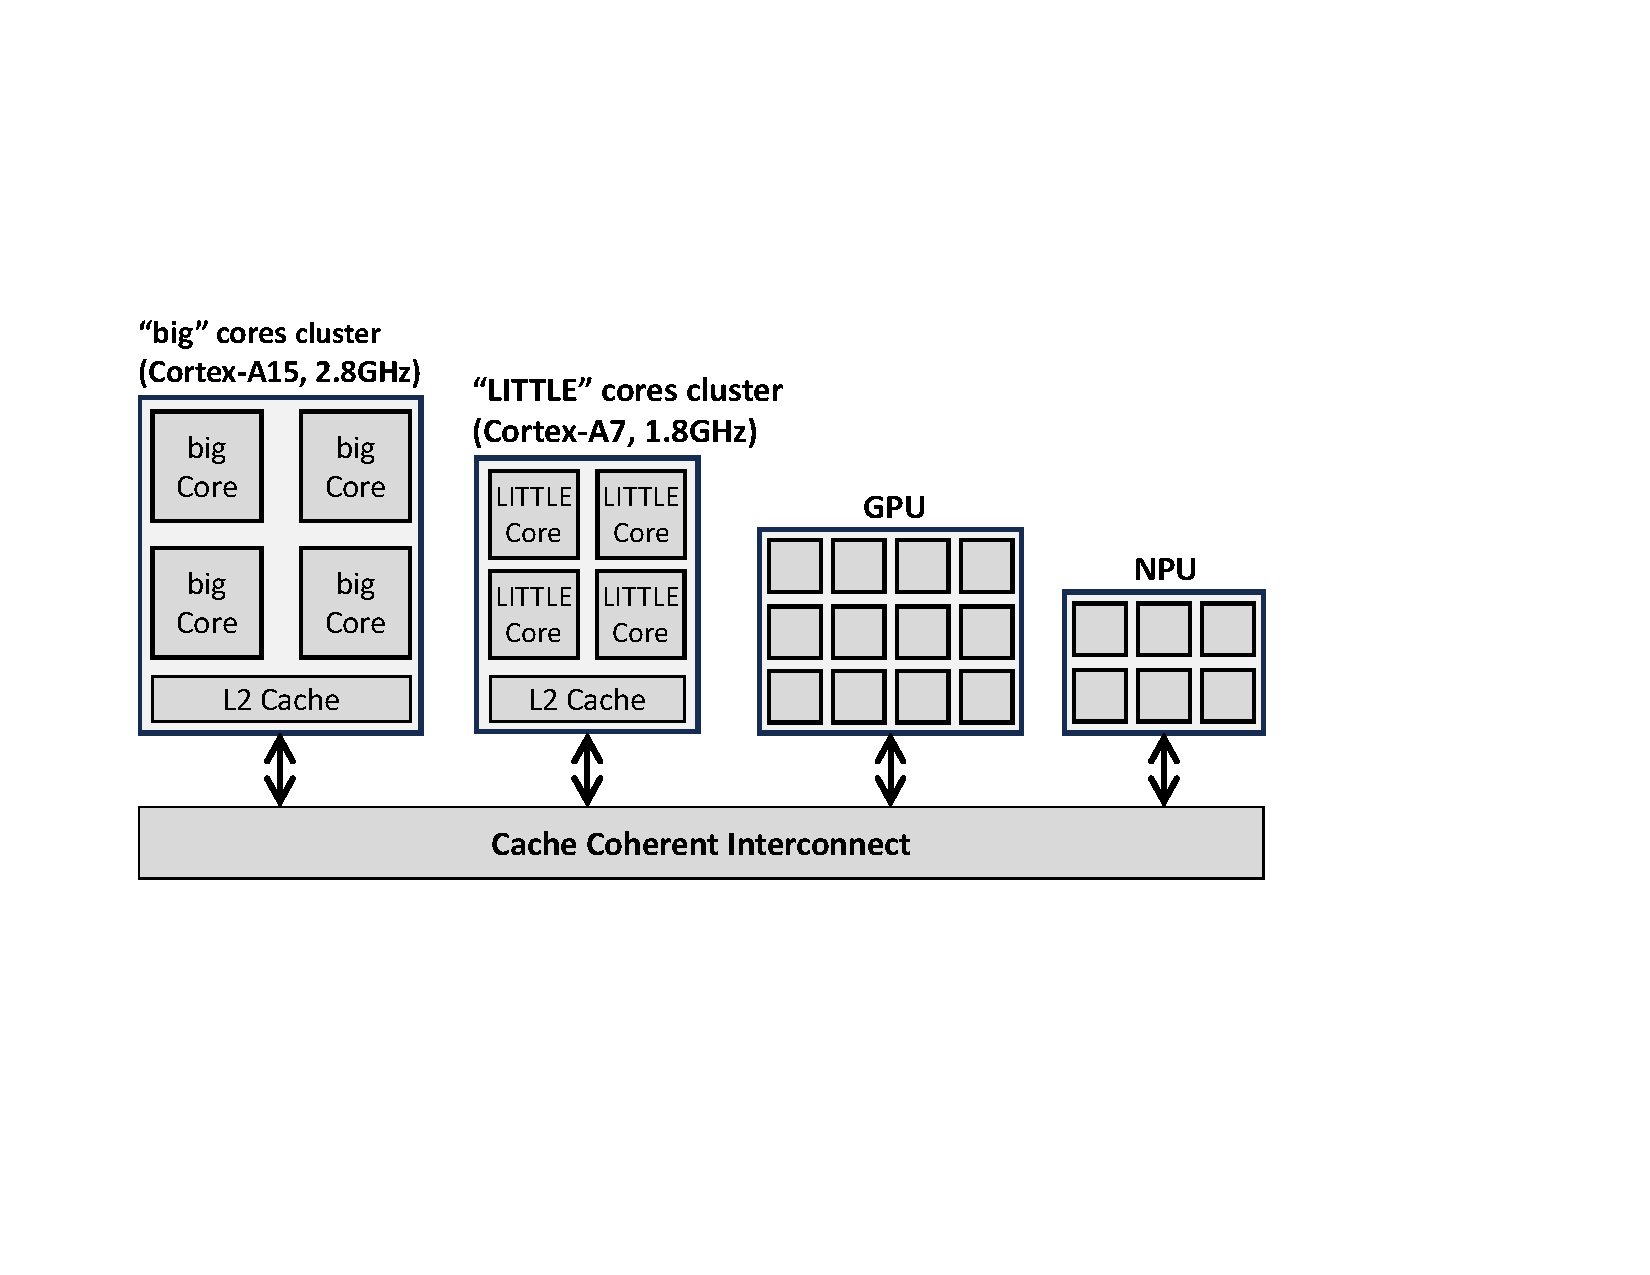
\includegraphics[width=1\linewidth]{figs/bigLITTLEArchitecture.pdf}
\vspace{1mm}
\caption{The ARM big.LITTLE architecture: overview}
\label{fig:bigLITTLEArchitecture}
\end{subfigure}

\begin{subfigure}{.95\columnwidth}
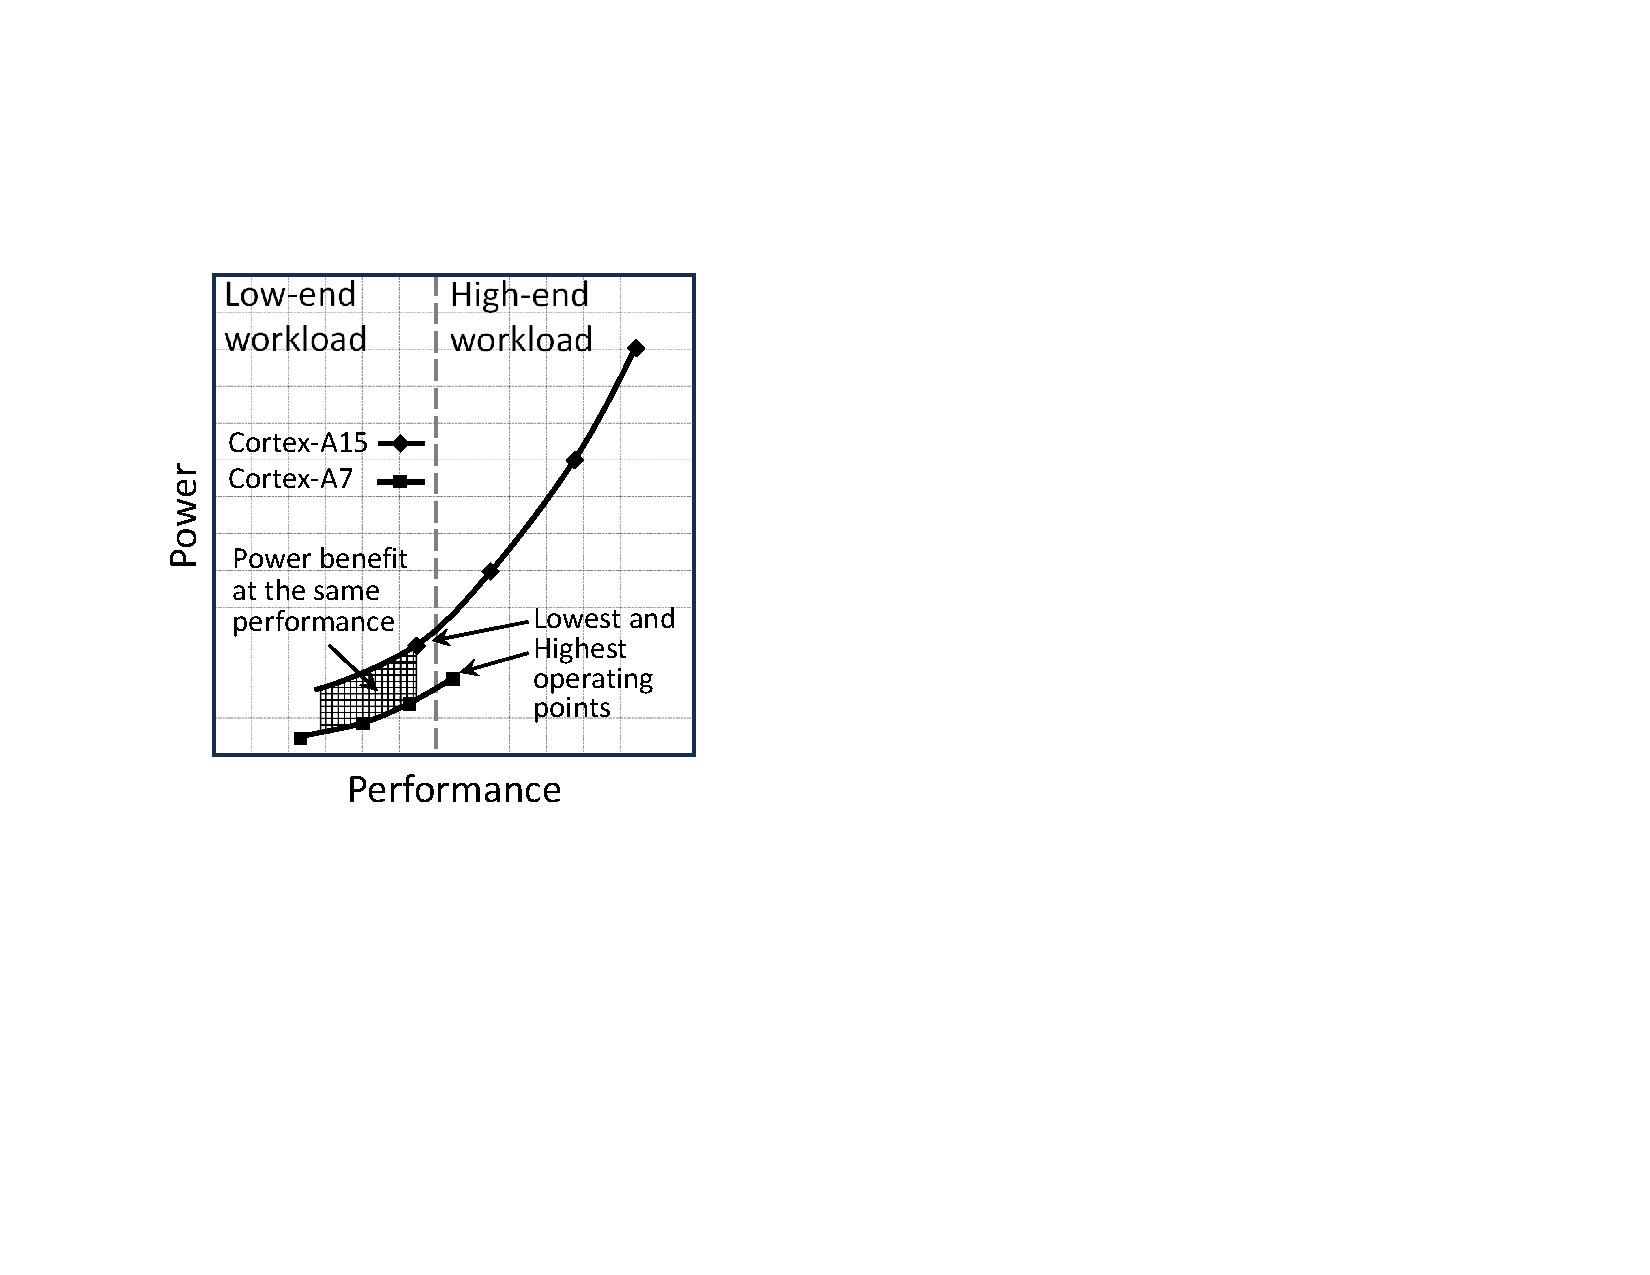
\includegraphics[width=.4\linewidth]{figs/CortexA15vsA7Comparison.pdf}
\vspace{1mm}
\caption{Power/performance trends}
\label{fig:CortexA15A7Comparison}
\end{subfigure}
\caption{Heterogeneous architecture: example with Cortex-A15 and Cortex-A7}
\end{figure*}

\begin{figure}
\centering
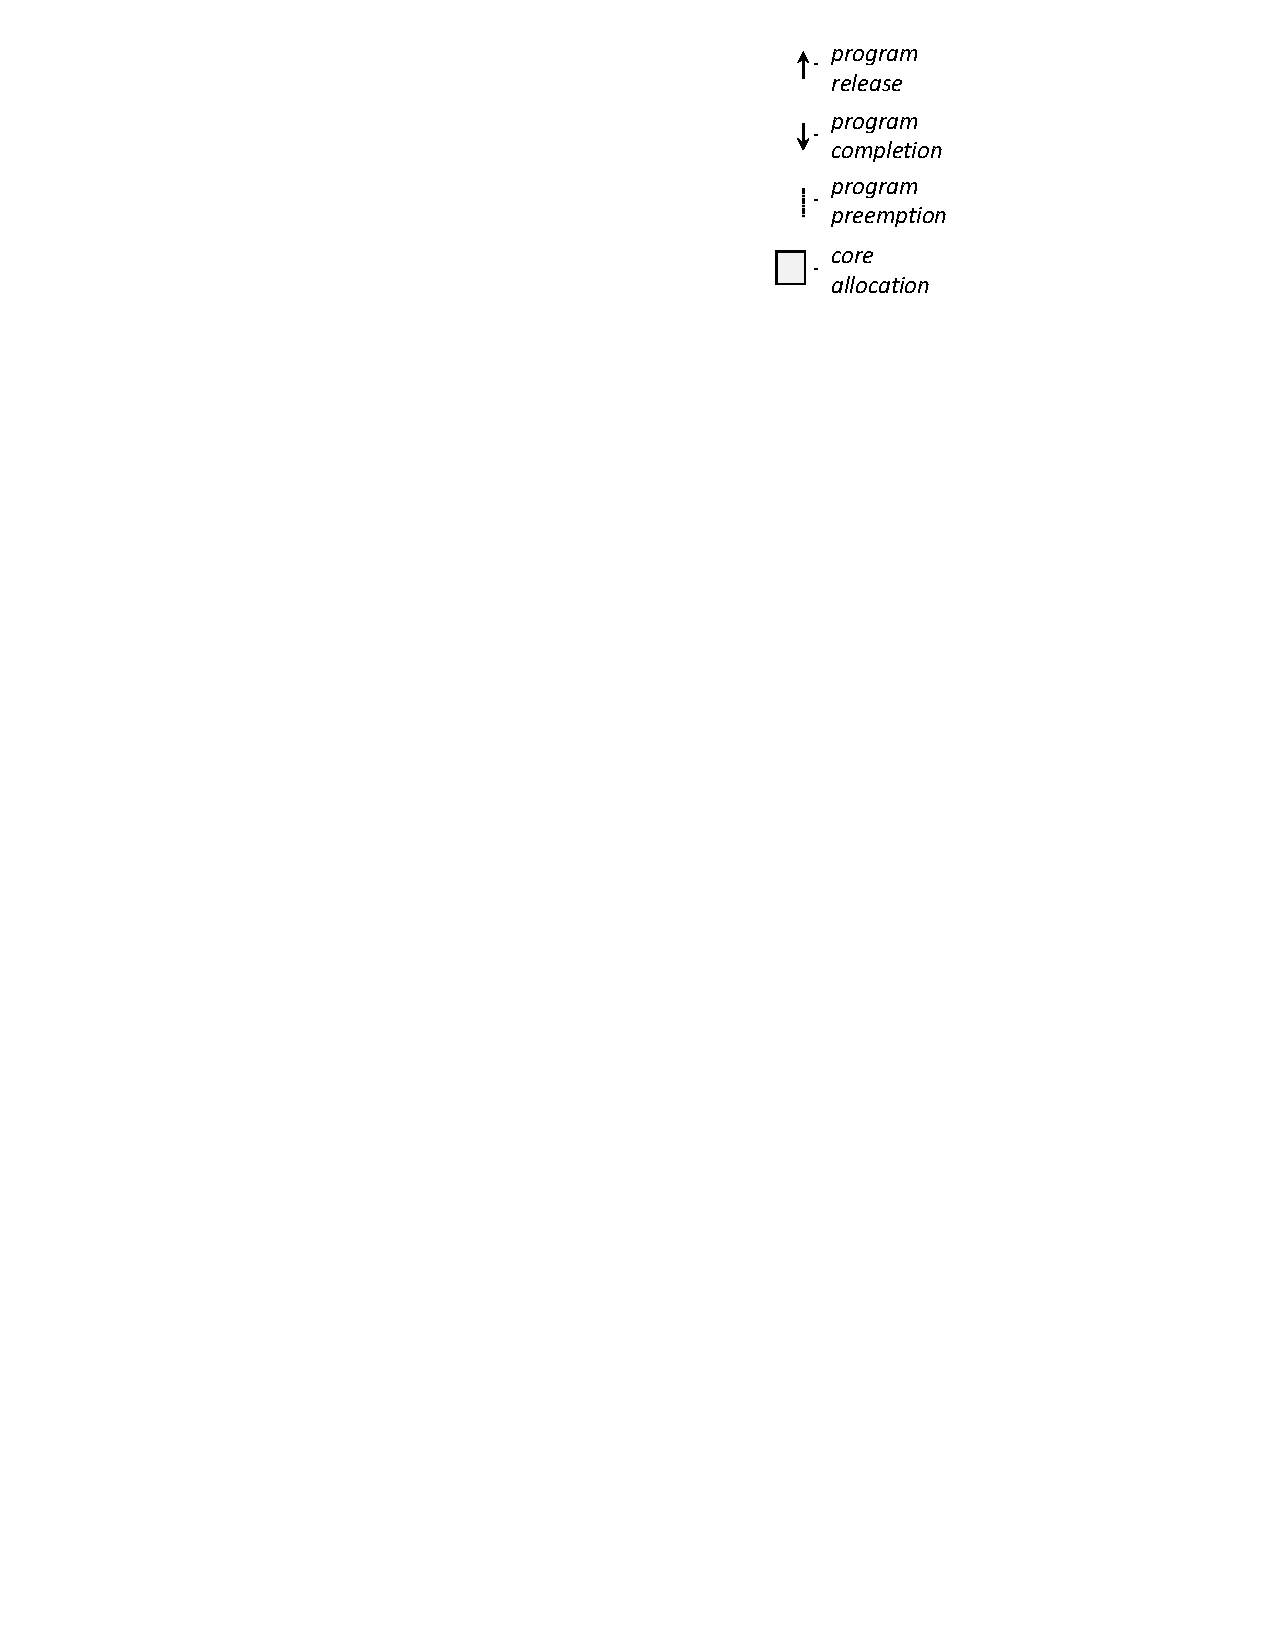
\includegraphics[width=.18\columnwidth]{figs/notation.pdf}
\caption{Graphical notation for Fig.~\ref{fig:twoSchedulesExample},~\ref{fig:singleProcessorCase},~\ref{fig:s1PreemptionMigration}, and~\ref{fig:executionMetrics}}
\label{fig:notation}
\end{figure}

The figures, as well as the rest of the manuscript, rely on the graphical notation in Fig.~\ref{fig:notation}.




\section{Contribution} 
We propose a novel approach for heterogeneous scheduling. It is based on traversing state-transition graphs of executed programs. More specifically, our contributions are:
%
\begin{itemize}
\item A theoretically optimal heterogeneous scheduler. Unlike other existing schedulers, our one addresses not only programs response time, but also energy consumption;
\item Scheduling heuristics, which make scheduling decisions significantly faster than an optimal scheduler. We also demonstrate  that some heuristic is near-optimal;
\item A prototype C++ tool implementing all our schedulers;
\item A thorough comparison of all proposed schedulers.
\end{itemize}
%
At the moment our schedulers do not account for preemption and migration overheads. However, the proposed state-transition graph methodology is easily extendable to such more realistic scenarios.

\begin{figure*}
\begin{minipage}{.7\columnwidth}%
\begin{subfigure}{\linewidth}
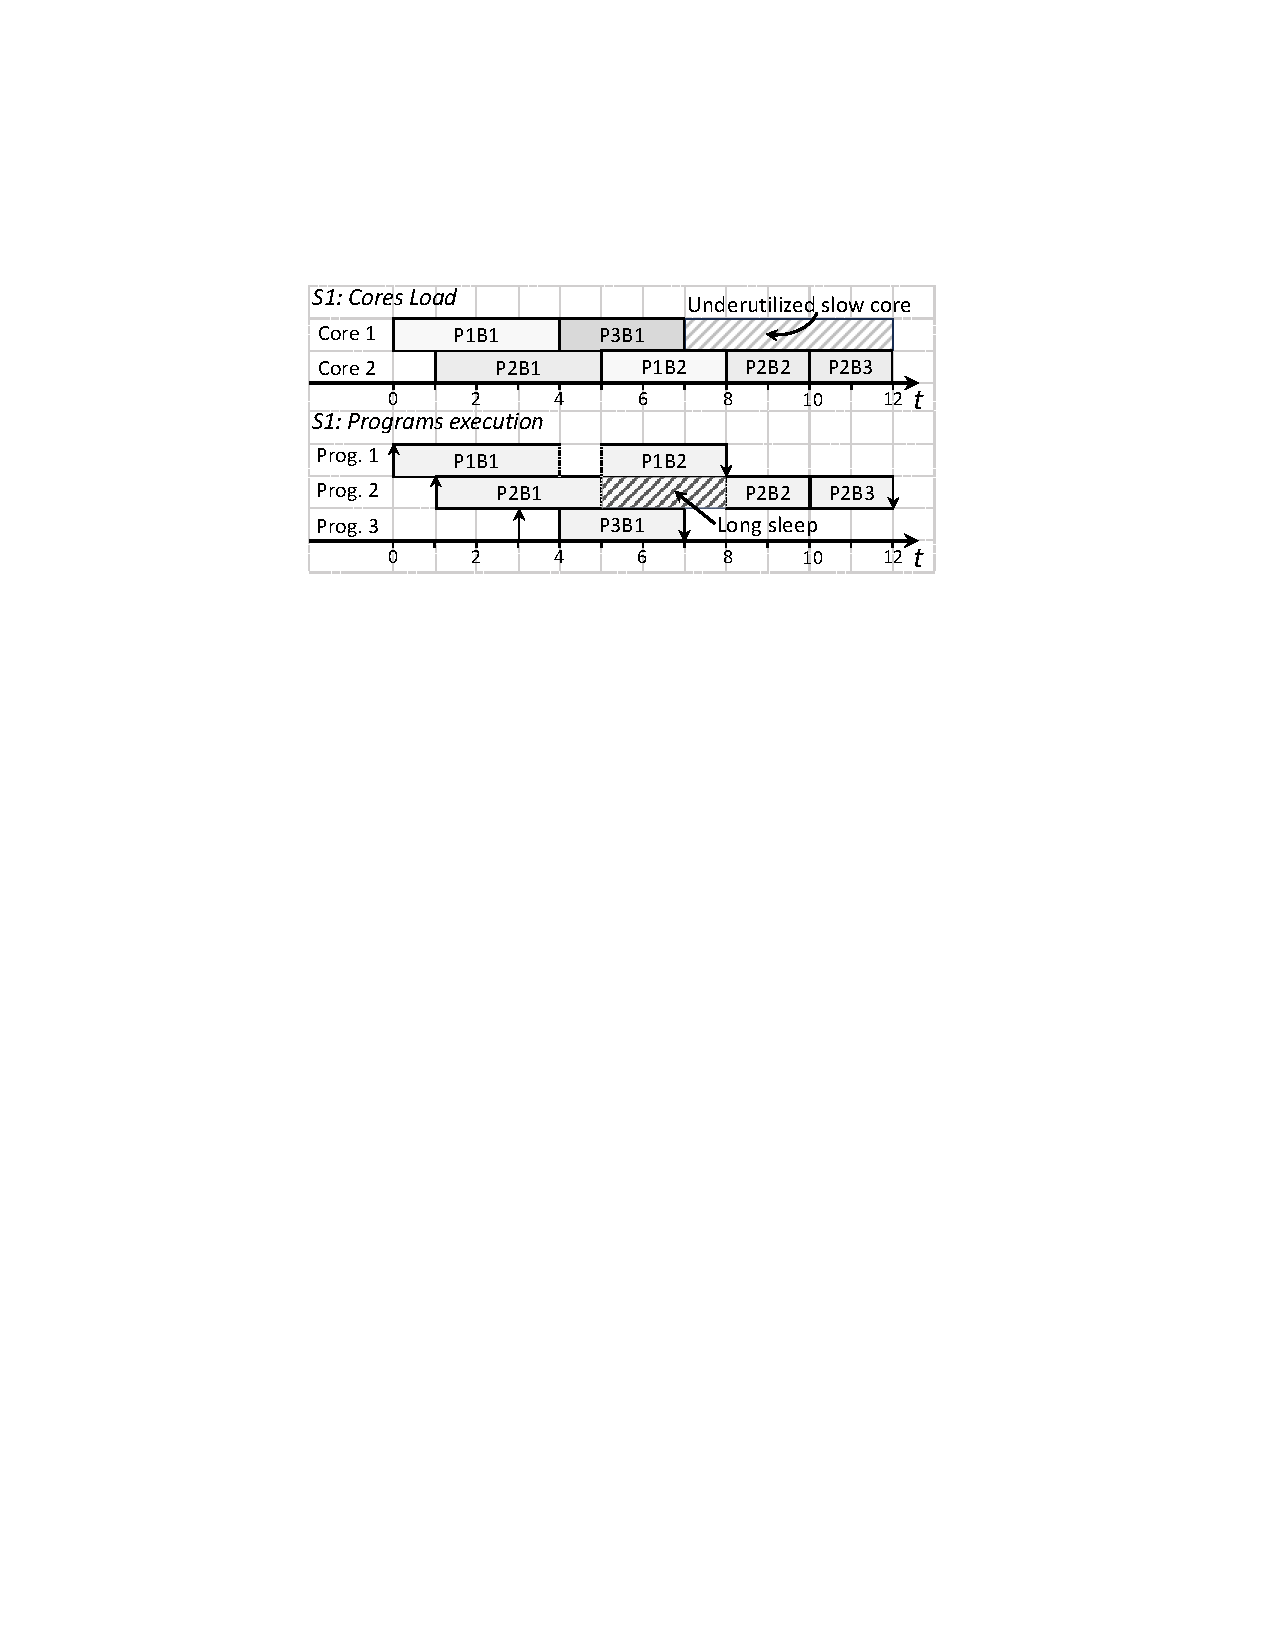
\includegraphics[width=\linewidth]{figs/s1.pdf}
\caption{Schedule S1: programs execution}
\vspace{3mm}
\label{fig:s1}
\end{subfigure}

\begin{subfigure}{\linewidth}
\centering
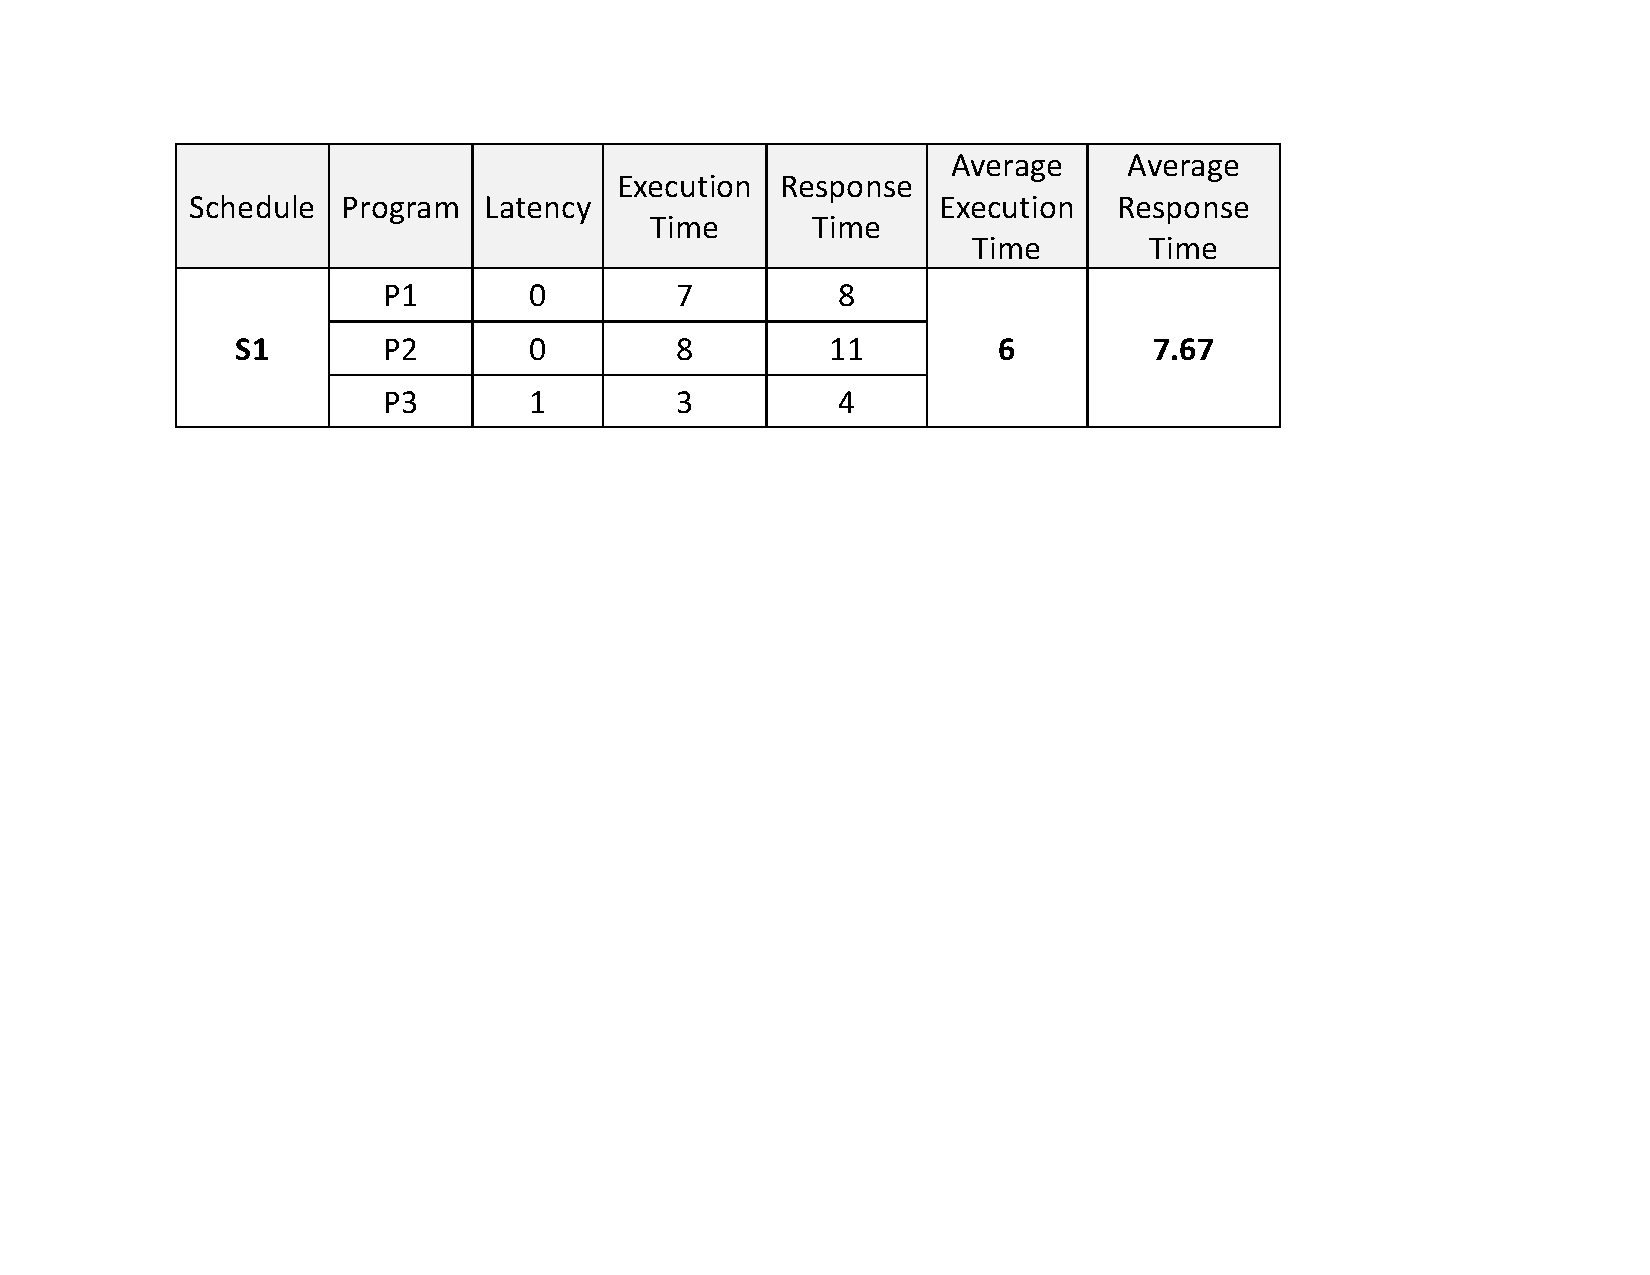
\includegraphics[width=\linewidth]{figs/s1Metrics.pdf}
\caption{S1: time performance metrics}
\vspace{1mm}
\label{fig:s1Metrics}
\end{subfigure}
\end{minipage}

\begin{minipage}{.7\columnwidth}%
\begin{subfigure}{\linewidth}
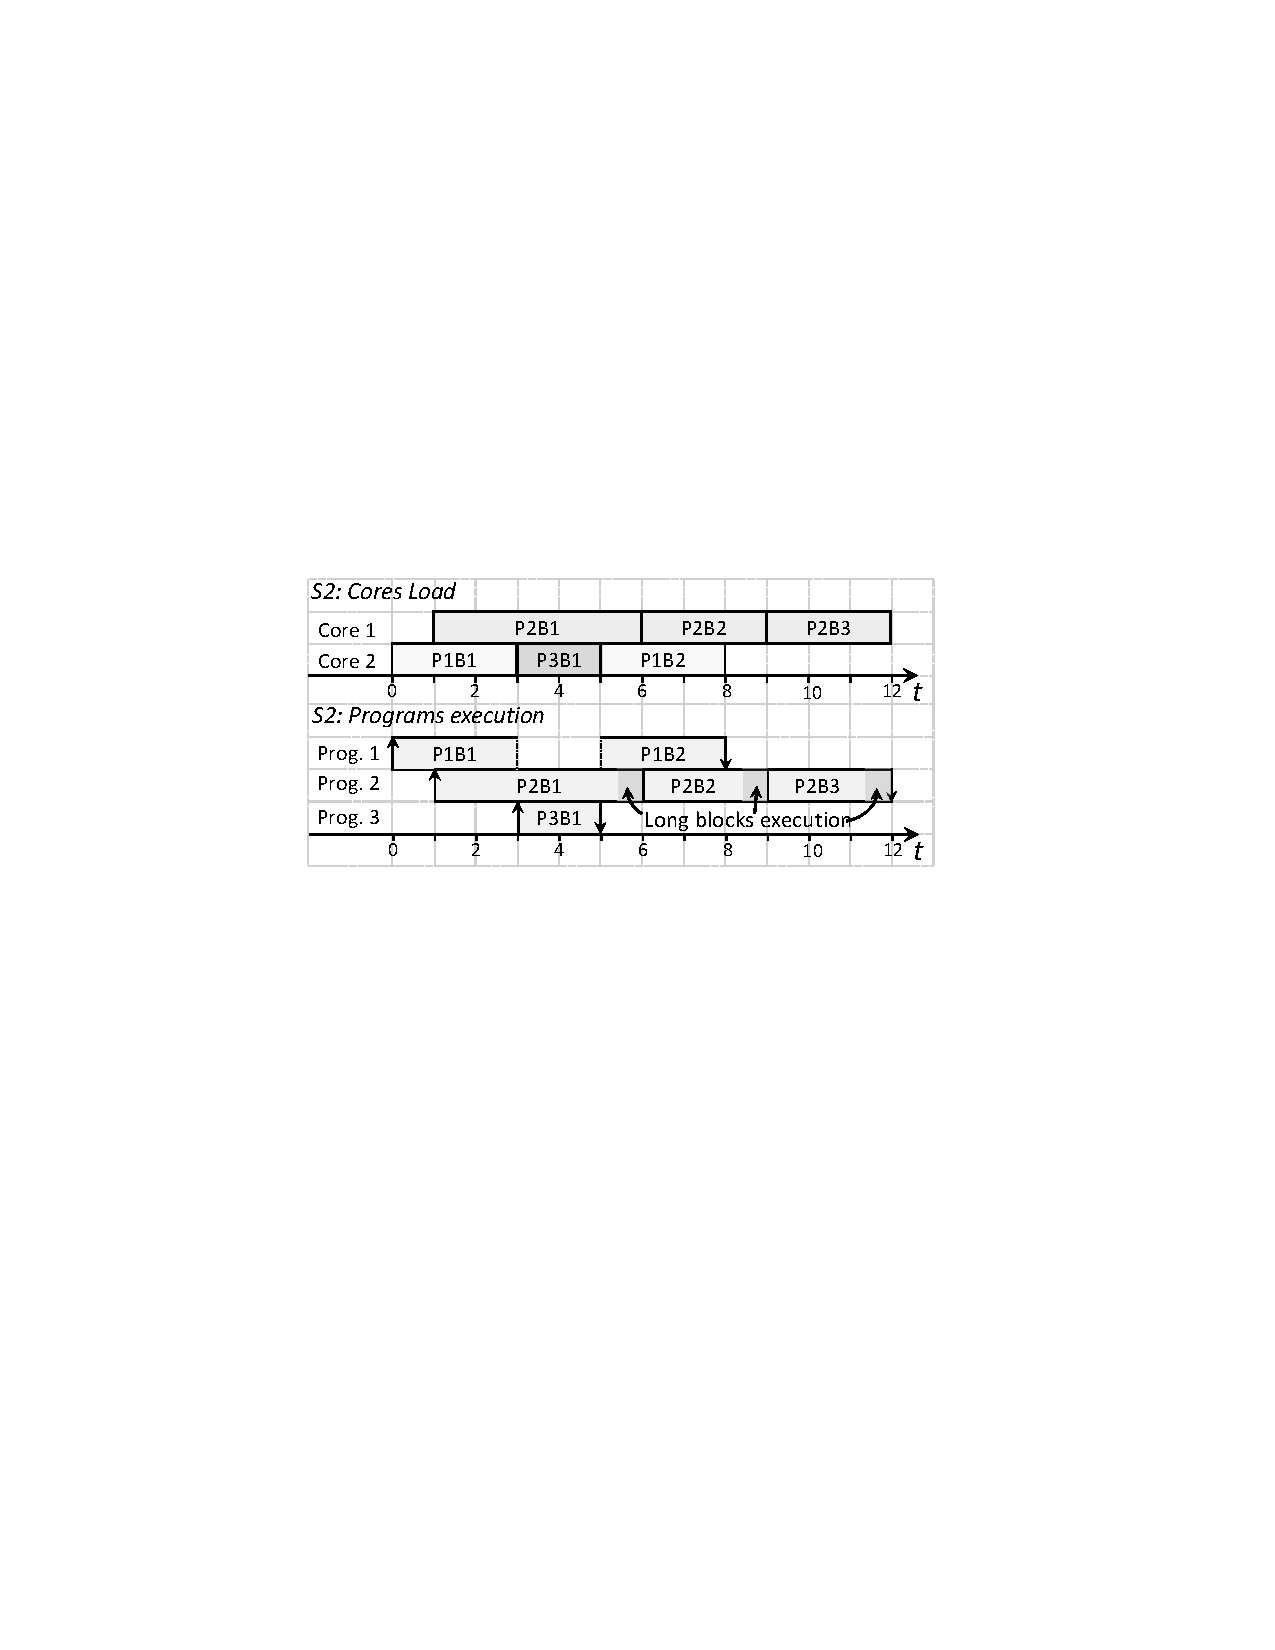
\includegraphics[width=\linewidth]{figs/s2.pdf}
\caption{Schedule S2: programs execution}
\vspace{3mm}
\label{fig:s2}
\end{subfigure}

\begin{subfigure}{\linewidth}
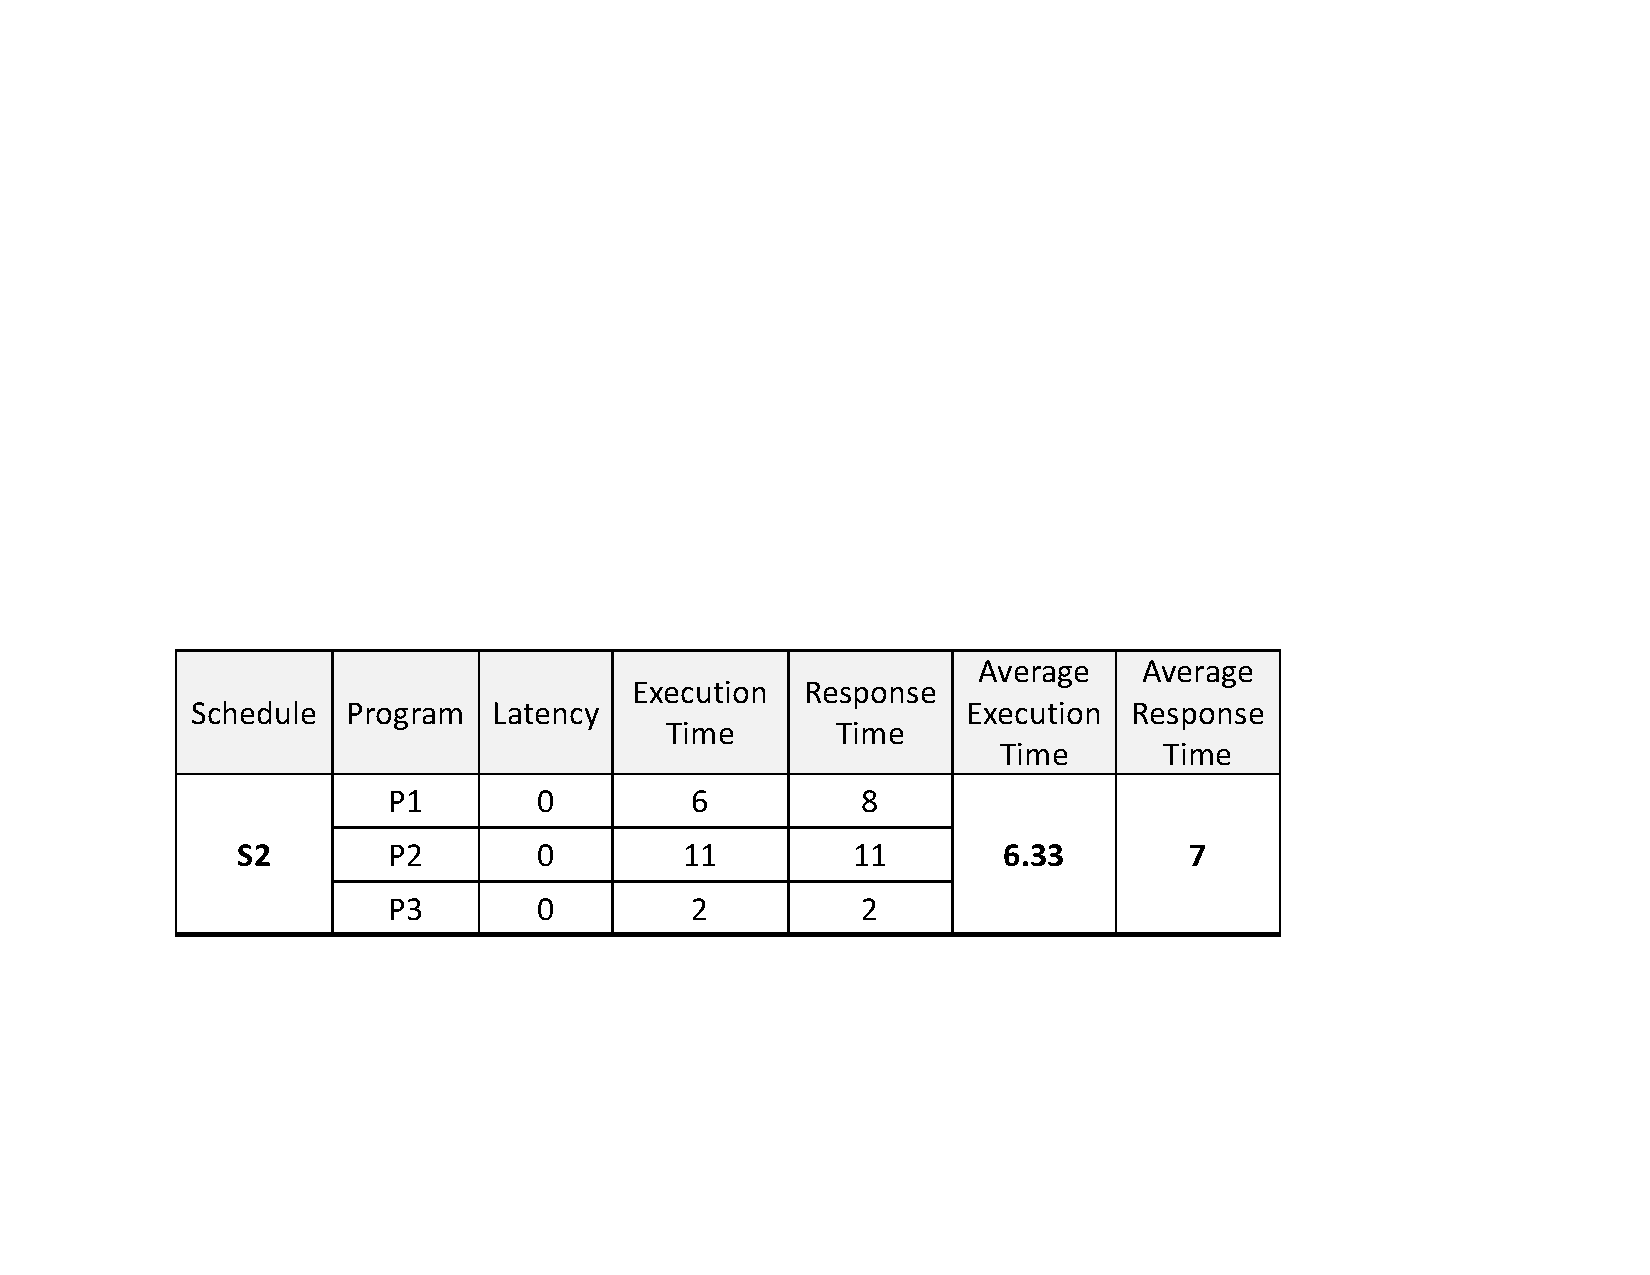
\includegraphics[width=\linewidth]{figs/s2Metrics.pdf}
\caption{S2: time performance metrics}
\vspace{1mm}
\label{fig:s2Metrics}
\end{subfigure}
\end{minipage}%

\caption{Sample execution schedules for programs from Table~\ref{tab:demandExample} (no migrations and preemptions considered)}
\label{fig:twoSchedulesExample}
\vspace{-3mm}
\end{figure*}

\section{Organization} 
The rest of the paper is organized as follows. In the first sections we describe the necessary background for our analysis. After introducing the heterogeneous scheduling problem and a toy example in Chapter~\ref{chap:intro}, we next, in Chapter~\ref{chap:systemModel}, introduce the system model for a heterogeneous computing platform and programs processing requirements. Then, in Chapter~\ref{chap:processorSchedulingStrategies} we revise multiprocessor scheduling strategies, which serve as the basement for our refined scheduler. We dedicate Chapter~\ref{chap:efficiencyMetrics} to discuss various programs performance metrics to be considered in the analysis, both reflecting time and energy consumption. After providing the necessary preliminaries, we derive our optimized heterogeneous scheduler. In Chapter~\ref{chap:optimizedHeterogeneousScheduling} we describe analytically our optimized scheduling driven by the notion of a state-transition graph. After that, in Chapter~\ref{chap:evaluation}, we report the evaluation results for our approach through a set of experiments. Finally, in Chapter~\ref{chap:conclusion}, we conclude our work by discussing potential directions for optimizing our heterogeneous scheduler.
